% 1.1 Problem Statement
\section{Research Problem and Motivation}
\label{sec:intro_prob_form_motiv}
\index{Intro!Research Problem and Motivation}

\begin{figure}[t]
	\centering
	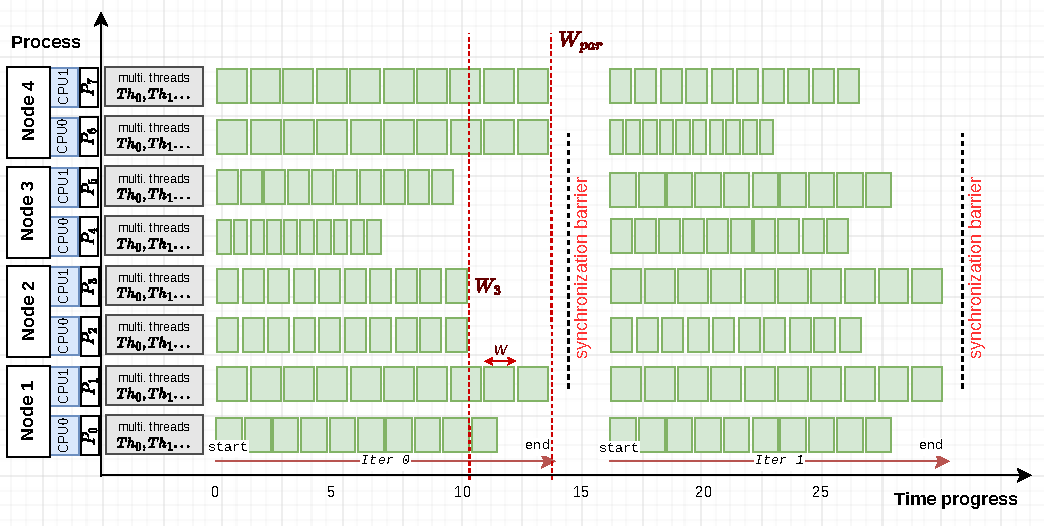
\includegraphics[scale=0.7]{./pictures/introduction/intro_problem_formulation.pdf}
	\caption{An illustration refers to a real iterative execution with load imbalance in task parallel application, running on 4 compute nodes, 2 processes per node, and multiple threads per process.}
	\label{fig:intro_prob_formulation}
\end{figure}

We illustrate the load imbalance context in Figure \ref{fig:intro_prob_formulation} to explain the problem formulation intuitively. This figure reveals a similar case shown in Figure \ref{fig:intro_usecase}, load imbalance at runtime on 4 compute nodes. Again with the x, y coordinates, the x-dimension shows the time progress, the y-dimension shows the involved processes within compute nodes but in more detail with the threads executing tasks on each process. We intend to highlight this illustration as a realistic execution and refer to a hybrid parallel programming model in practice, multiprocessing + multithreading. A modern processor today is mostly multicore architecture; hence, a process mapped to a processor can create multiple threads pinned to multiple corresponding cores within that processor.\\

Suppose we use MPI to leverage communication between processes, then the hybrid model is known as MPI+X \cite{rabenseifner2006mpiomp}. In Figure \ref{fig:intro_prob_formulation}, each process, e.g., $P_{0}$, $P_{1}$, indicates an MPI process (also called MPI rank). One MPI process can spawn multiple threads to execute tasks denoted by \texttt{multi.threads} ($Th_{0}$, $Th_{1}$, and so on). The term ``multiple threads'' refers to many threads, where a thread is the segment of a process. While processes are mostly isolated, threads share memory and data. Therefore, we assume tasks are automatically scheduled and fairly executed within a process. An imbalance at runtime comes from different processes across different compute nodes, not within a process. Before every execution phase, each process is assigned a given number of tasks, and this assignment normally follows the partitioning algorithm of an application called a given task distribution on processes. In Figure \ref{fig:intro_prob_formulation}, we highlight the first execution phase (denoted by Iteration 0 or \texttt{Iter 0} for short), where tasks belonging to process $P_{1}$, $P_{6}$, and $P_{7}$ are executed slower than the others, causing the load imbalance.\\

For comprehensive analysis, we formulate the problem as follows. Given $T$ tasks in total, the tasks are indexed from $\{0,...,(T-1)\}$ and distributed among $P$ processes before execution. When $T$ is mentioned as a set, we can understand it as $\{0,...,(T-1)\}$; when $T$ is mentioned as an integer number, it is the total number of tasks. Each process is denoted by $P_{i}$, where $i$ in the range of $\{0,...,(P-1)\}$. Similar to $T$, $P$ can be mentioned as the number of processes if it is an integer number or the set $\{0,...,(P-1)\}$. A scheduled task is atomic and runs on a specific thread until termination. Tasks, load values, and evaluation metrics are summarized in detail below.
\begin{itemize}
	\item $T_{i}$: a set of assigned tasks for process $P_{i}$, e.g., $T_{1}$ is the set of assigned tasks belonging to process $P_{1}$. When $T_{i}$ is mentioned as an integer number, it indicates the number of tasks assigned to process $P_{i}$.

	\item $w$: the load value of a task in general. The value of $w$ is also called a wallclock execution time and $w > 0$. When we refer to a load of a particular task in a set $T_{i}$ of process $P_{i}$, $w$ can be attached with an index $j$, which means task $j$ belongs to the set $T_{i}$. Overall, $T_{i}$ is a subset of $T$, and all tasks in $T_{i}$ belong to the set $T$. Therefore, a particular value $w_{j}$ must be $> 0$ and $j$ $\in$ $\{0,...,(T-1)\}$. The standard deviation between the values of $w$ determines the type of tasks, uniform or non-uniform. Uniform tasks indicate the tasks with approximate load values, while non-uniform tasks indicate the tasks with different load values resulting in a high standard deviation of the load values of tasks. In Figure \ref{fig:intro_prob_formulation}, the length of green boxes highlights the length of $w$. For this illustrated case, we can say that the load values of tasks in a process are uniform, but different tasks in different processes are non-uniform.
	
	\item $L_{i}, \forall i \in P$: the total load of process $P_{i}$, where $L_{i} = \sum_{j \in T_{i}} w_{j}$.
	
	\item $W_{i}, \forall i \in P$: the wallclock execution time of process $P_{i}$. Unlike $L_{i}$, $W_{i}$ indicates the completion time of process $P_{i}$ when all tasks are done. The execution of all tasks here indicates that they are executed in parallel by multiple threads in process $P_{i}$. Both $L_{i}$ and $W_{i}$ at the end will reflect the imbalance ratio. Figure \ref{fig:intro_prob_formulation} marks $W_{3}$ as an example to indicate $W_{i}$.
	
	\item $W_{par}$: the parallel wallclock execution time known as the completion time, makespan, or application time, $W_{par} = max_{i \in P}(W_{i})$. For example, in Figure \ref{fig:intro_prob_formulation} $W_{par}$ is determined by process $P_{6}$, $P_{7}$ at \texttt{Iter 0}.
	
	\item $R_{imb}$: imbalance ratio, $R_{imb} = \frac{W_{max}}{W_{avg}} - 1 = \frac{W_{par}}{W_{avg}} - 1$, where $W_{max}$ is the maximum wallclock execution time ($max_{i \in P}(W_{i}) = W_{par}$), and $W_{avg}$ is the average value ($avg_{i \in P}(W_{i})$). Alternatively, we can also calculate $R_{imb}$ via the total load values such as $R_{imb} = \frac{L_{max}}{L_{avg}} - 1$.
\end{itemize}

If $R_{imb} \approx 0$, there is no imbalance. If $R_{imb}$ is greater than or equal to a certain threshold, $R_{imb}$ is determined imbalance at runtime. For example, users define a threshold $0.2$, and $R_{imb} \geq 0.2$ is determined as an imbalance. In this case, $W_{par}$ is seen as unoptimized. Our work targets reducing the values of $R_{imb}$ and $W_{par}$.\\

In our context, task migration is the only way to perform dynamic load balancing because tasks are already distributed among compute nodes. At runtime, we cannot share or add more computing resources in distributed memory systems. Otherwise, the technology must be changed to enable sharing resources across separate machines.\\

As mentioned in Section \ref{sec:intro_overview}, the previous approaches are mostly based on two schemes of dynamic load balancing: master-worker and work stealing. When considered in principle, all of these approaches comprise four components to their operations \cite{xu1996load}. The four components can be explicit or implicit, including:
\begin{itemize}
	\item Load measurement: indicates monitoring, checking either the load status or the execution speed.
	\item Information exchange: indicates the operations of status exchange among processes. This operation helps to synchronize the execution status to calculate imbalance ratio.
	\item Initiation rule: implies when to initiate a balancing operation. It can be initialized by overloaded processes or underloaded processes or periodically at runtime.
	\item Load balancing operations: implies the actions used to balance the load, e.g., task migration, thread/process migration. There might be different rules \cite{xu1996load} for making decisions on these actions.

\end{itemize}

\begin{figure}[t]
	\centering
	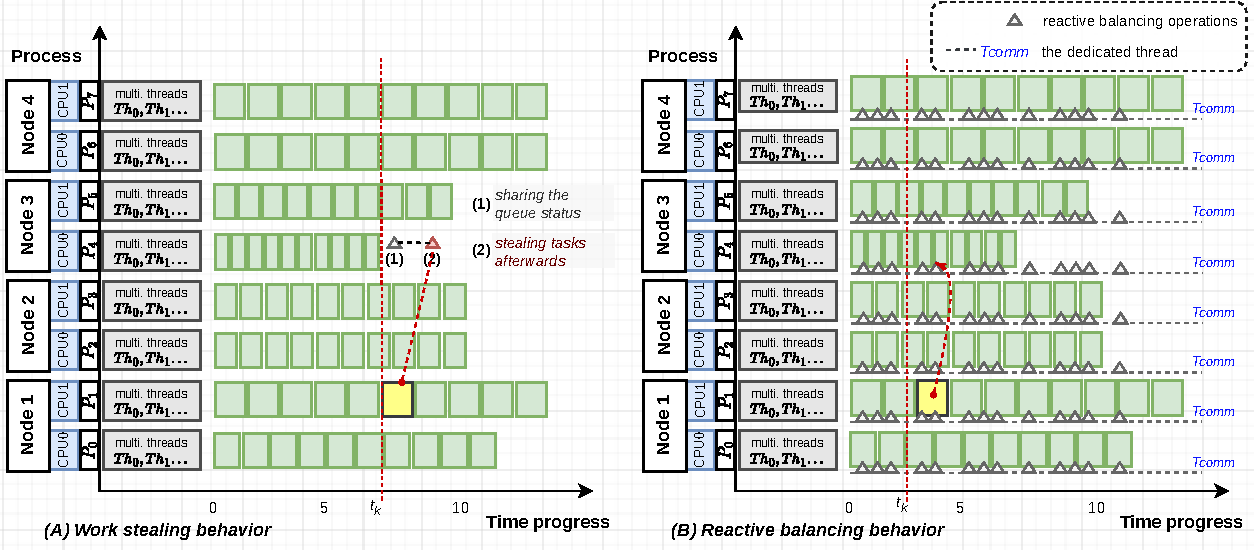
\includegraphics[scale=0.65]{./pictures/introduction/intro_motiv_workstealing_vs_reactlb.pdf}
	\caption{Behaviors of work stealing and reactive load balancing.}
	\label{fig:intro_motiv_workstealing_vs_reactlb}
\end{figure}

A master-worker scheme works as a centralized scheme, where the master is a central point, and workers wait to receive commands from the master. It is easy to manage load and control the balance of load, but it is challenging to scale up the number of distributed memory machines.\\

Work stealing is more relevant in our imbalance context. However, if we take communication overhead in distributed memory machines into account, the behavior of work stealing can be limited by the components of ``information exchange'' and ``load balancing operations''. The reasons are that tasks have to be migrated, and the behaviors of work stealing can make it too late to steal tasks. In a detailed inspection, these behaviors can refer to different variants. They are classified as follows.
\begin{itemize}
	\item Passive: indicates work stealing in distributed memory systems, which has several proposed approaches for HPC clusters \cite{ravichandran2011wsmulticorhpc} and also in-depth analysis of stealing-tasks behavior through performance modeling \cite{gast2021analysis}. The algorithms and behaviors of work stealing in distributed memory differ from shared memory because the global operations, such as synchronization primitives, caching, or coherence protocols, often result in high overhead and latency. Another point is a contention that may occur when multiple thieves try to steal tasks from the same victim process \cite{paudel2013meritdistws}. Therefore, in most algorithms for distributed memory, the decision of stealing tasks is taken when an idle process exists. Basically, the idle process sends out a steal request when its local queue is empty. Depending on a specific algorithm, the busy processes may also be in charge of responding to steal requests before a task is stolen. Thereby, we consider the behavior of processes performing work stealing in distributed memory systems as a passive action.\\
	
	 For illustration, Figure \ref{fig:intro_motiv_workstealing_vs_reactlb} (A) shows work stealing applied to the imbalance case illustrated in Figure \ref{fig:intro_prob_formulation}. The x-axis again represents time progress during execution, and the y-axis highlights the labels of compute nodes, processes with their executing-tasks threads. At time $t_{k}$, process $P_{4}$ is idle, then it needs to mainly perform: (1) sharing/exchanging the idle status with other processes, (2) stealing tasks afterward if one of the overloaded processes responds to the request. When an agreement is made, process $P_{4}$ steals a task from process $P_{1}$. The stolen task is denoted by the yellow box. As we can see, these behaviors can be too late if communication overhead is dominant, leading to missed requests, an unexpected number of stolen tasks, or even some overloaded processes that are not handled fairly.
	
%\noindent In work stealing, the bottleneck is obviously with migration overhead, and the time to make stealing decisions is too late. For reactive load balancing, we must assume that a shortcoming period is valid about the imbalance for reacting to task offloading. Even when we make reactive decisions, it might be challenging to decide how many tasks should be offloaded at once. Besides, choosing or pairing an offloader with a victim might be unfair and incorrect because of no prior knowledge about load at runtime, especially in high imbalance cases. Therefore, these points have motivated the thesis as follows:

	\item Active: indicates the behaviors as seen in the state-of-the-art approaches. Instead of waiting until a process is idle, we attempt to send tasks actively from one process to another beforehand, if the imbalance is speculatively observed or predicted. Depending on how much information we have in a specific context, we can divide ``active'' into two variants:
		\begin{itemize}
			\item Reactive: emphasizes responding to situations after certain conditions are satisfied. When an imbalance is detected periodically, this reacts with a decision of migrating or not migrating tasks. In particular, prior knowledge about load values is not needed. This reaction is only based on the most current status of execution and short-period speculation. After that, we perform these reactive operations repeatedly and continuously. Therefore, task migration here does not mean stealing tasks but offloading tasks\footnote{``Offload'' and ``migrate'' might be used interchangeably in this thesis} and we refer to reactive task offloading \cite{klinkenberg2020reactmig}.
			\item Proactive: emphasizes taking actions in advance based on anticipating/predicting the future. This means we know more details about the imbalance situation, e.g., how much imbalance and load value are. Therefore, proactive task offloading means offloading tasks earlier and more controllable than reactive task offloading.
		\end{itemize}
	
\end{itemize}

Several reactive load balancing approaches have been proposed \cite{Klinkenberg2020ChameleonReactLB} \cite{Samfass2021ChameleonReactRepLB}. These approaches continuously monitor the execution status instead of waiting for an empty queue. The monitored status information helps calculate imbalance ratio ($R_{imb}$) based on the queue length. Then, we can determine which process executes tasks slow and which process is fast. Following that, we can offload tasks from a slow process to a fast process reactively.\\

``Slow'' and ``fast'' imply overloaded and underloaded processes. For example, Figure \ref{fig:intro_motiv_workstealing_vs_reactlb} (B) shows a reference implementation with MPI+OpenMP \cite{rabenseifner2009hybrid}. One thread per process is dedicated to be a communication thread (called $Tcomm$). $Tcomm$ is used to overlap communication and computation. For reactive load balancing, $Tcomm$ on each process monitors the execution speed, shares this information with other processes, and calculates the imbalance ratio. These operations are continuous and repeated. If an imbalance is detected over a given condition, we can offload tasks promptly from a slow process to a fast one. For example, at time $t_{k}$ in Figure \ref{fig:intro_motiv_workstealing_vs_reactlb} (B), the imbalance is detected, and the reactive decision is made earlier than work stealing shown in Figure \ref{fig:intro_motiv_workstealing_vs_reactlb} (A). In this case, assuming that process $P_{1}$ is slow and process $P_{4}$ is fast as a good victim for offloading tasks. Victims in work stealing indicate the overloaded processes whose tasks are stolen. In reactive approaches, victims indicate the underloaded (fast) processes where tasks are offloaded to. The downside of reactive load balancing can be wrong speculation because we rely only on the most current status of execution speed. Periodically, reactive task offloading can be decided incorrectly under high imbalance cases. Besides, performance can be affected at the end when tasks are offloaded with an inappropriate number or wrong victims. \\

The limitations of work stealing and reactive load balancing motivate us to investigate a new proactive approach. In principle, our idea tries to tackle dynamic load balancing with the following constraints:
\begin{itemize}
	\item Performance slowdown at runtime causes imbalance, which is unknown before running applications. This refers to the inherent variation in supercomputer architectures with the design of today multicore CPUs. Acun et al. use compute-intensive kernels and applications to analyze the variation among processors in different supercomputers \cite{acun2016variturboboost}. They observe that there is an execution time difference of up to 16\% among processors under enabling Turbo Boost. The intrinsic differences in the chips’ power efficiency are the culprit behind the frequency variation. A similar work is from Weisbach et al. \cite{weisbach2018hwvariation}; they also show six orders of magnitude difference in relative variation among CPU cores across different compute platforms such as Intel x86, Cavium ARM64, Fujitsu SPARC64, IBM Power.
	\item Communication overhead is a bottleneck for exchanging execution status and migrating tasks. The communication overhead in distributed memory systems comes from:
		\begin{itemize}
			\item Latency ($\lambda$): time between sending and receiving the head of a message, where $\lambda$ does not depend on the size of a message.
			\item Delay time ($d$): time for transmitting an entire message between two nodes, where $d$ depends on the size of a message.
		\end{itemize}
	\item At runtime, we lack load information as well as system performance information to estimate better when, where, and how many tasks should be migrated at once.
\end{itemize}
